\section{Alternative Interventions}
\label{sec:alternatives}

Given that tail nodes benefit most from SSL, a natural question is whether targeted interventions can improve upon global SSL. We evaluate two categories: selective CL variants and non-CL baselines.

\paragraph{Selective CL does not outperform global CL.}
We test three targeting strategies: DegreeGatedCL (CL only on nodes with $\deg \leq 5$), RandomCL (CL on random 30\% of nodes), and UncertaintyCL (CL on the 30\% most uncertain nodes via MC dropout). Figure~\ref{fig:selective} shows that none consistently outperform GlobalCL on cold-edge AUC.

\begin{figure}[t]
    \centering
    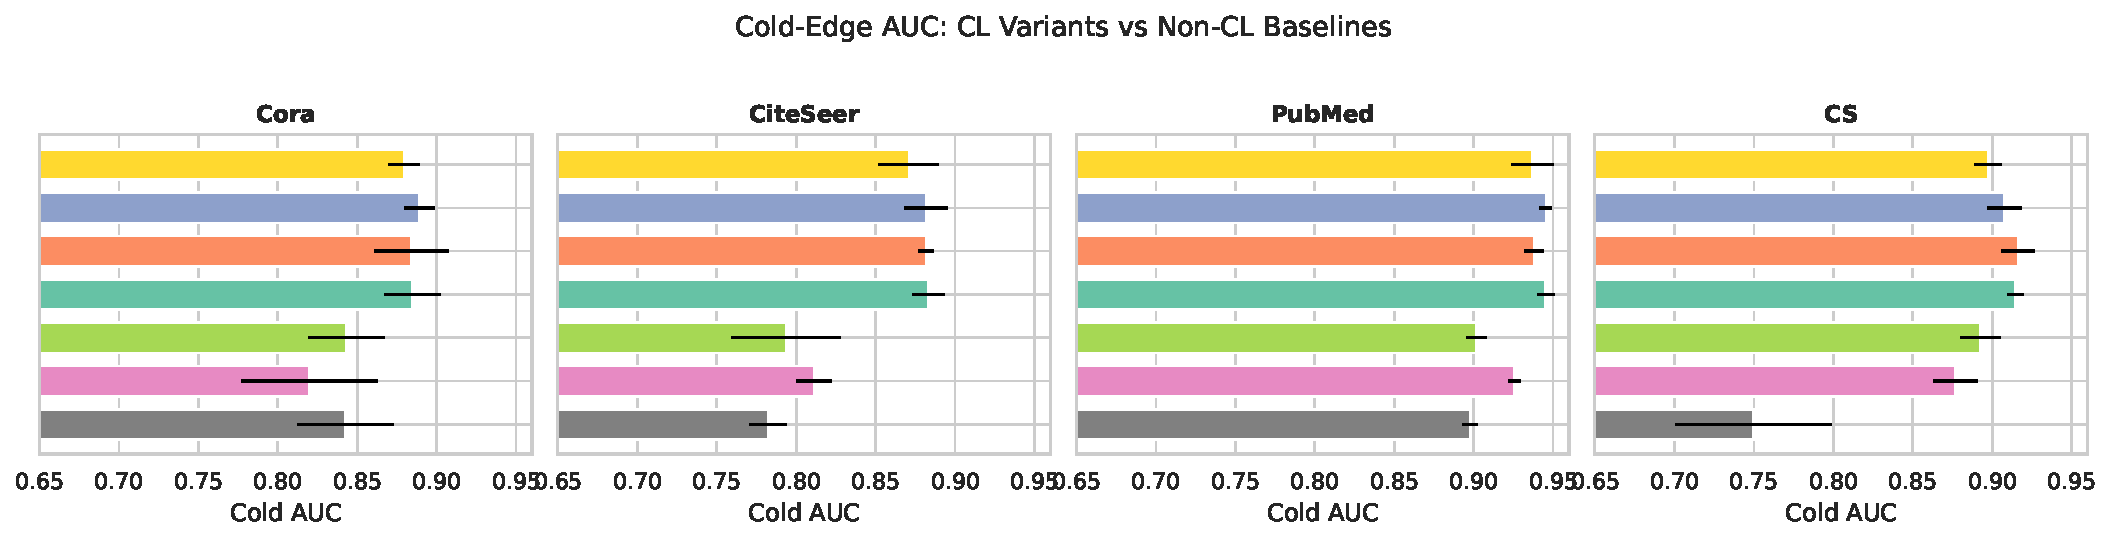
\includegraphics[width=\linewidth]{figures/fig4_selective.pdf}
    \caption{Cold-edge AUC across methods. All CL variants perform similarly, substantially outperforming non-CL baselines. Selective targeting provides no advantage over global CL.}
    \label{fig:selective}
\end{figure}

Across all datasets, GlobalCL, DegreeGatedCL, and RandomCL achieve statistically indistinguishable cold-edge AUC (differences within 1 std). UncertaintyCL is marginally worse, likely due to the noise introduced by periodic uncertainty re-estimation during training. This negative result suggests that the tail benefit of CL arises from \emph{global} representation regularization---reshaping the entire embedding space---rather than from node-specific contrastive invariances.

\paragraph{Non-CL baselines are substantially weaker.}
Loss reweighting ($3\times$ weight on cold edges) and focal loss ($\gamma=2$) both improve tail performance over Vanilla, but the gains are 2--5$\times$ smaller than SSL methods. On CS, Reweight improves cold AUC by +12.7\% over Vanilla, while GlobalCL improves by +16.5\%. On Cora, Reweight provides no cold improvement ($-$2.3\%), while GlobalCL provides +4.2\%.

This gap confirms that SSL offers a qualitatively different form of regularization that cannot be replicated by simply paying more attention to tail examples during supervised training. The CL benefit extends beyond hard-example mining: it changes how the model represents the entire graph, with disproportionate benefits for under-determined (low-degree) regions.
